\documentclass[12pt]{article}
\include{amsfonts,amssymb,amsmath,amsthm,txfonts,pxfonts,mathrsfs,enumitem}
\usepackage{ctex}
\usepackage[headheight=15pt,paperwidth=8.5in, paperheight=11in]{geometry}
\usepackage{lastpage}
\usepackage{fancyhdr}
\usepackage{float}
\usepackage{indentfirst}
\usepackage{geometry}
\usepackage{enumitem}
\usepackage{graphicx}
\newcounter{teamnumb}
\setcounter{teamnumb}{1234}
\ttfamily{
\lhead{Team\ \# \theteamnumb}\rhead{Page \thepage\ of \pageref{LastPage}}}
\cfoot{}
\renewcommand{\headrulewidth}{0pt}
\pagestyle{fancy}
\begin{document}
\section*{Summary}
\thispagestyle{empty}
 \clearpage
\setcounter{page}{1}
\section{Statement and Clarification of Problem}
\section{Assumptions and Rationale/Justification}
\subsection{Postulations}
	The important postulations we make includes the following:\par
	We consider the colony to be self-support, every household is also considered to be the owner of the company. The whole economy produces a single kind of identical products using two inputs: Labor and Capital.
	We also make a very strong assumption that the market price of everything is equal to its value. In other words, real wage equals to $MPL$(Marginal product of labor). Every household's income is also the production of the company.	
\subsection{Individual Traits}
	We construct our model from two perspectives. First it is assumed that each individual has the following basic traits that distinguish them from each other: gender, race, age, education\footnote{We measure 'education' by an integer starting from 1 and every year's study augments 'education' by 1.}, capital\footnote{It's necessary at this point to clarify the economy system we model. First, everything related to money is measured in its real value. In other words, there is no inflation involved in this model, everything from wages to GDP is in real term rather than nominal term.}. We also introduce  randomness by adding a random factor. From the factor above we derive the three important behaviors of an individual: willingness to work, marginal propensity to consume and productivity. In the following graph, it is demonstrated how individual traits determine these behaviors.
\begin{figure}[H]
\centering
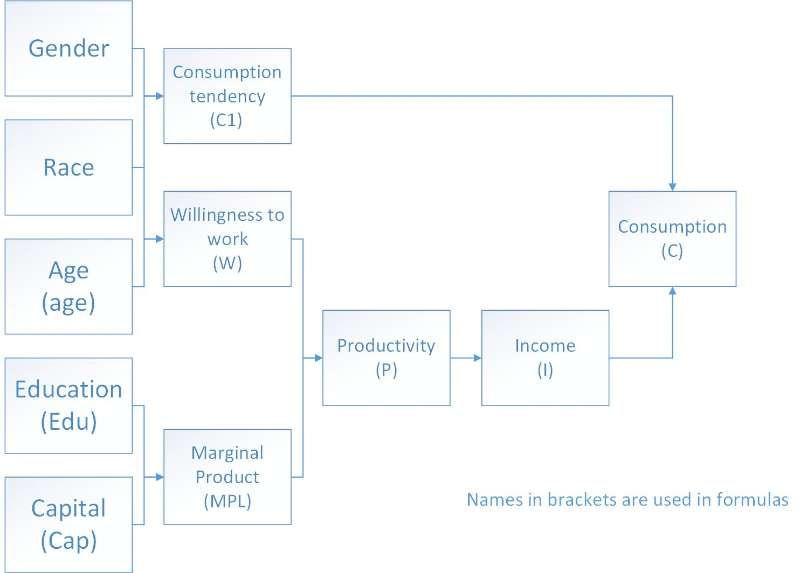
\includegraphics[scale=.65]{Individual.jpg}
\end{figure}	
\subsubsection{Productivity}
	We assume that productivity comes from the product of willingness to work and marginal product of labor($MPL$). Let the random factor be $R$(indicating talent, idiosyncrasy and etc), $f(age)$ be a function of age\footnote{$f(age) = 0$ when age is below 18 or over 52. Within the range of $(18, 52)$, $f(age)$ gradually grows as age increase from 18, and reaches apex at $35$, then gradually drops back to zero at 52.}. We suppose individual productivity takes the form:
\begin{equation}
P = W \times MPL = W \times R \times f(age) \times \sqrt{Cap * Edu}
\end{equation}
	The formula is mainly derived from intuition and basic macroeconomics knowledge, yet we may still substantiate it in the following sense. First, productivity is positively related to talent and capital. Meanwhile talented people may take better use of capital, so $R$ should be a multiplier. Second, education is an indicator of the skill level one possess, which is directly related to marginal product of capital, so $Cap \& Edu$ should take the form of $Cap \times Edu$. Third, due to diminishing marginal product, we adopt the form of square root for simplicity while the form has negative second derivative, complying with the principle of diminishing return.\par
\subsubsection{Consumption}
	We reckon that individual consumption($C_t$) consists of basic consumption($C_b$) and extra consumption($C_e$). Basic consumption is the minimum consumption for each individual to survive. Government has the obligation to support those who can't afford basic consumption due to either unemployment or disability. \par
	The simplest model for consumption would be:
\begin{equation}
C_t = C_b + C_e = C_b + C_1 \times I \times (1 - taxRate)
\end{equation}
where $C_t$ is linear with respect to after-tax income.
\subsubsection{Willingness to work}
	For simplicity, we split colonists into two races: Producer and Innovator. We suppose that innovator has a significantly greater willingness-to-work than producer. Willingness-to-work is also an index of working time,
\section{Plans with respect to different timespan}
\subsection{Short Term Plan(��һ��)}
In our model, we use average income(we have deducted tax out)to indicate the priority factor, which is a natural and convenient choice.\par
For education, we develop an education level to describe how many years a person have studied.It is an integer, which increases by year if one's still at school.We presume that if a person is at school, he will gain education.This presumption ignore the different effect of studying between different people, as simplification. One's education level contributes to his production, just like in our real life, an educated person is more likely to gain skill and knowledge and be a workforce of high quality.Based on this assumptions, average education level is a fair factor to demonstrate the education level of the society as a whole.\par
For social equality, which is thorny to evaluate in our real life.In order to simplify this condition, we first consider a series of factor contributes to a person's happiness, as we have stated before(in section ???). Then, we define equality by the standard deviation of happiness of every person in this society. The definition reflects that if gap between different people(different in income, education, degree of happiness) is widening, people in this society will feel less equal.\par
In the initiate course of settling down of economy system, no doubt, productivity is the most important. As a result, the most important indicator of social progress at first is Income, measured by GDP. The greater the GDP, the higher its growth rate, the better the society will be.\par
For the sake of promoting GDP in the first several years, a large enough population is needed. At the same time, Population quality is a non-negligible factor. Higher education level contributes to the production and development. The age structure is also a crucial factor. Youth and mid-aged should be of proper ratio so that there will be enough people working while the society will not step into the aging process. A proper age structure will lead to reasonable birth rate and death rate, which is conducive to the long-term development and prosperity of society.
\section{������}
For social equality, which is thorny to evaluate in our real life.In order to simplify this condition, we first consider a series of factor contributes to a person's happiness, as we have stated before(in section ???). Then, we define equality by the standard deviation of happiness of every person in this society. The definition reflects that if gap between different people(different in income, education, degree of happiness) is widening, people in this society will feel less equal.\par
As a model, we are supposed to evaluate the society by multi-factor comprehensively considering. For this goal, we define social happiness(H) by the equation below:
\begin{equation}
H=\sum_{i = 1}^N h_i -\lambda*N*Eq
\end{equation}
In this Equation, $h$ means a person's happiness. The summation is for every person alive in the society.
$N$ is the amount of  people and Eq is the equality of the whole society. $\lambda$ is an artificial coefficient, which is related to the inclination of policy makers. The more the equality of colony are embraced, the larger the value of  $\lambda$ \par
The definition of the aggregate happiness of the whole society measure both individual happiness and the variance of happiness between individuals. A unfair distribution of happiness may causes social instability and a low sense of security, which may deplete social happiness. Therefore, we use the standard deviation to measure the negative effect of inequality and subtract it from the sum of individual happiness to obtain the final outcome of the aggregate social happiness.

\section{Conclusions}
\end{document}
